\documentclass[12pt,a4paper]{article}
\usepackage[utf8]{inputenc}
\usepackage[czech]{babel}
\usepackage[T1]{fontenc}
\usepackage{amsmath}
\usepackage{amsfonts}
\usepackage{amssymb}
\usepackage{graphicx}
\usepackage[left=3cm,right=3cm,top=3cm,bottom=3cm]{geometry}
\author{Ondřej Zelenka}
\begin{document}

\pagenumbering{gobble}

\section*{Závěrečná olympiáda z fyziky, LMFS 2017 - starší}

\subsection*{1. Nabitý prostor (12 bodů)}
V trojrozměrném prostoru vzhledem ke sférickým souřadnicím $r,\theta,\phi$ mějme statické rozložení elektrického náboje takové, že příslušný elektrostatický potenciál má tvar
\begin{equation}
\Phi\left(r,\theta,\phi\right) = U_0\cdot\frac{e^{-r/l}}{r}.
\end{equation}
Určete rozložení náboje v prostoru.\\
\emph{Nápověda} Jsou i jiné způsoby rozložení náboje než objemové!

\subsection*{2. Doletět, či nedoletět (10 bodů)}
Nejmenovaný diktátor nejmenované Koreje se špatně vyspal. Rozhoduje se, které město na Zemi zničit. Jeho rakety doletí do vzdálenosti $d = 6000$ km. Kolik kilometrů jim bude chybět do zničení Prahy? Geografické souřadnice:\\
\begin{tabular}{l r r}
Praha: & 50$^\circ$ 5' s. š., & 14$^\circ$ 25' v. d.\\
Pchjongjang: & 39$^\circ$ 2' s. š., & 125$^\circ$44' v. d.
\end{tabular}\\
Uvažujte, ze střela letí po nejkratší trajektorii přímo nad povrchem ideální kulové Země o poloměru 6378 km. Kartézské souřadnice z geografických získáte jako
\begin{subequations}
\begin{align}
x &= r\cos\vartheta\cos\phi\\
y &= r\cos\vartheta\sin\phi\\
z &= r\sin\vartheta.
\end{align}
\end{subequations}

\subsection*{3. kosmická rychlost (8 bodů)}
Určete 3. kosmickou rychlost $v_{III}$, tedy rychlost potřebnou k úniku tělesa na povrchu Země z gravitačních vlivů Země i Slunce. Hmotnost Země je $m_Z = 5.97\cdot 10^{24}$ kg, Slunce $m_S = 1.99\cdot 10^{30}$ kg, vzdálenost Země od Slunce je 1 AU = $149\cdot 10^6$ km.

\subsection*{4. Kopa nábojů (9 bodů)}
Rozmístíme 162 stejně velkých nábojů $Q\neq 0$ do vrcholů pravidelného 162-úhelníku o délce strany $a$. Přidáme jeden náboj $q\neq 0$ do středu 162-úhelníku. Jaká na něj působí síla? Jaká na něj bude působit síla, když jeden z nábojů ve vrcholech odstraníme?

\subsection*{5. Koule v neviskózní kapalině (12 bodů)}
Dvě stejné kuličky ve vzduchu jsou nabité stejným elektrickým nábojem a jsou zavěšeny ve stejném bodě na dvou stejně dlouhých nitích, které spolu svírají úhel $2\alpha$ (náboj je dostatečně velký, aby se kuličky nedotýkaly). Nyní je ponoříme do benzenu o hustotě $\rho_b = 879$ kg$\cdot$m$^{-3}$ a relativní permitivitě $\epsilon_r = 2.3$ a po ponoření se úhel mezi nimi nezmění. Jaká je hustota kuliček?

\subsection*{6. Koule ve viskózní kapalině (14 bodů)}
Víťa má koule ve viskózní kapalině. V nádobě s ricinovým olejem o dynamické viskozitě $\eta$, která je ve stavu beztíže, urychlujeme kuličku o náboji $Q$ a poloměru $r$ homogenním a konstantním elektrickým polem $\vec{E}$, které míří ve směru osy $x$. Naopak ji brzdí Stokesův odpor $\vec{F} = -6\pi\eta r\vec{v}$, jedná se tedy o jednorozměrnou úlohu. Určete rychlost v ustáleném stavu (když se pohybuje rovnoměrně). Určete závislost polohy kuličky na čase, pokud se na počátku pohybuje ustálenou rychlostí a pole vypneme. Jak daleko se dostane? Vyhodnoťte pro $\eta = 987\cdot 10^{-3}$ Pa$\cdot$s, $r = 5$ mm, $E = 20$ V$\cdot$m$^{-1}$ a $Q = 0.1$ C.

\subsection*{7. Kulový kondenzátor (10 bodů)}
Určete kapacitu kondenzátoru tvořeného dvěma elektrodami ve tvaru soustředných kulových ploch o poloměrech $R_1$ a $R_2$.

\subsection*{8. CERN (8 bodů)}
Spočítejte velikost magnetické indukce, která zakřivuje trajektorii protonu o rychlosti $2c/3$ (nerelativisticky) v kruhovém urychlovači obvodu 27 km. Proton má náboj $q_p = 1.602\cdot 10^{-19}$ C a hmotnost $m_p = 1.67\cdot 10^{-27}$ kg.

\subsection*{9. Otáčení (9 bodů)}
Mějme vektorové pole v prostoru dané rovnicí
\begin{equation}
\vec{E}\left(x,y,z\right) = \left(\frac{4xy}{z},\frac{2x^2}{z},-\frac{2x^2y}{z^2}-z^3\right).
\end{equation}
%\begin{equation}
%\Phi = \frac{2x^2y}{z}-\frac{z^4}{4}
%\end{equation}
Rozhodněte, zda má potenciál, a pokud má, určete jej. (pokud nemá, nemusíte ho určovat)

\subsection*{10. Odporné odpory (8 bodů)}
Určete odpor zapojení na obrázku. Všechny zakreslené rezistory mají stejný odpor $R_0$. Namísto tří teček zapojení fraktálovitě (soběpodobně) pokračuje...\\\\
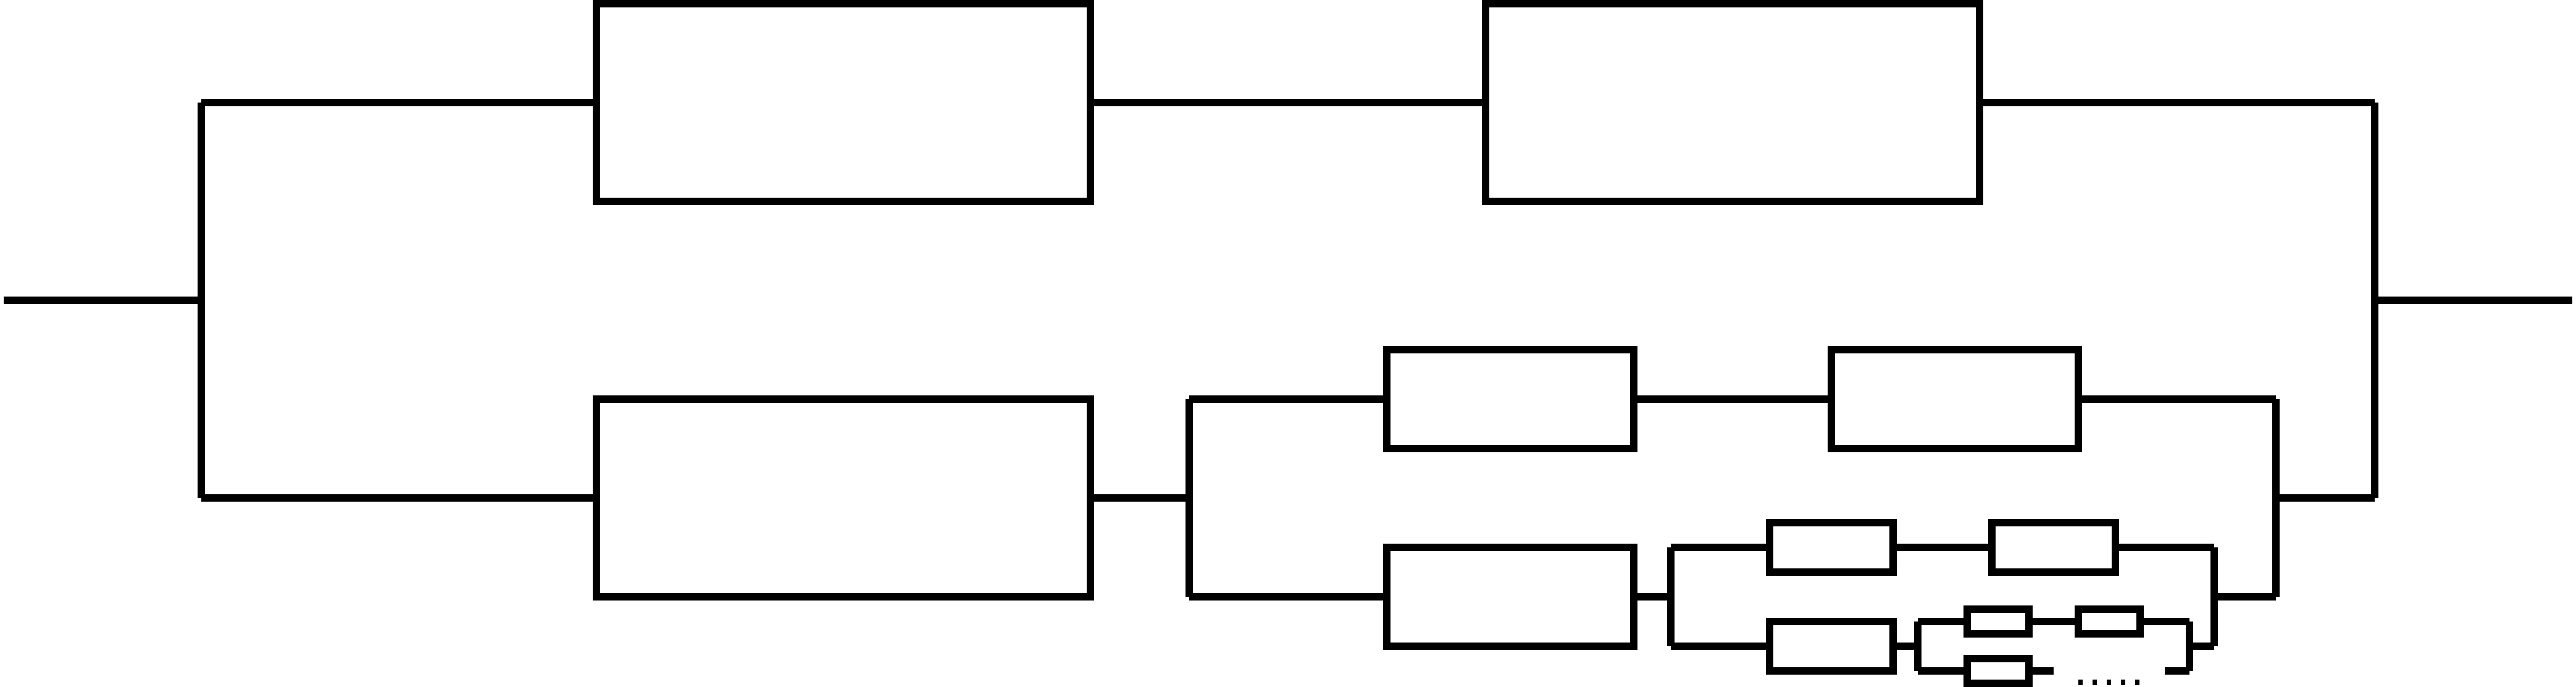
\includegraphics[scale=0.08]{img.png}

\end{document}